\documentclass[12pt,a4paper]{jsreport}
\usepackage{bm}
\usepackage[dvipdfmx]{graphicx}
\usepackage{ascmac}
\usepackage[hang,small,bf]{caption}
\usepackage[subrefformat=parens]{subcaption}
\captionsetup{compatibility=false}
\usepackage{geometry}
% ページの余白を1.25インチにする
\geometry{
    left=1.25truein,
    right=1.25truein,
    top=1.25truein,
    bottom=1.25truein,
}
\usepackage{etoolbox}
\patchcmd{\chapter}{\cleardoublepage}{}{}{}
\patchcmd{\chapter}{\clearpage}{}{}{}

\title{埋設されたパイプの位置・方向推定のための\\偏波感受型圧縮センシング}
\author{\\指導教員    廣瀬明教授 \\              夏秋嶺准教授\\
03-210499   高原陽太
}


\begin{document}
\maketitle
\tableofcontents
\clearpage
\chapter{はじめに}
\section{研究背景}
 工事のための地中調査を行う際、地中の埋設物の有無及びその状態を特定することは必須である。
特にガス管や水道管などが道路工事現場に埋まっているものの代表例として
挙げられる。そこで実際に工事を施工する前の調査段階でそれら埋設物の詳しい情報を得ておくことが重要となる。
\\ そのため電波を利用して地中を非破壊的に探知する地中レーダ(GPR)探査技術が用いられる。GPRは地中埋設物探査や遺跡調査、地下水流
調査など多くの応用分野を持つ\cite{radar1}\cite{radar2}。特定周波数帯の電磁波を地中に照射しその散乱特性を見る。
\\ 仕組みは以下の通りである。電磁波は地中を伝搬し、土壌中にて誘電率が異なる物質の境界面で散乱を起こす。そのため埋設物の材料物質と
土壌の誘電率の違いを利用して埋設物の検知を行う。


\begin{figure}[h]
    \begin{center}
     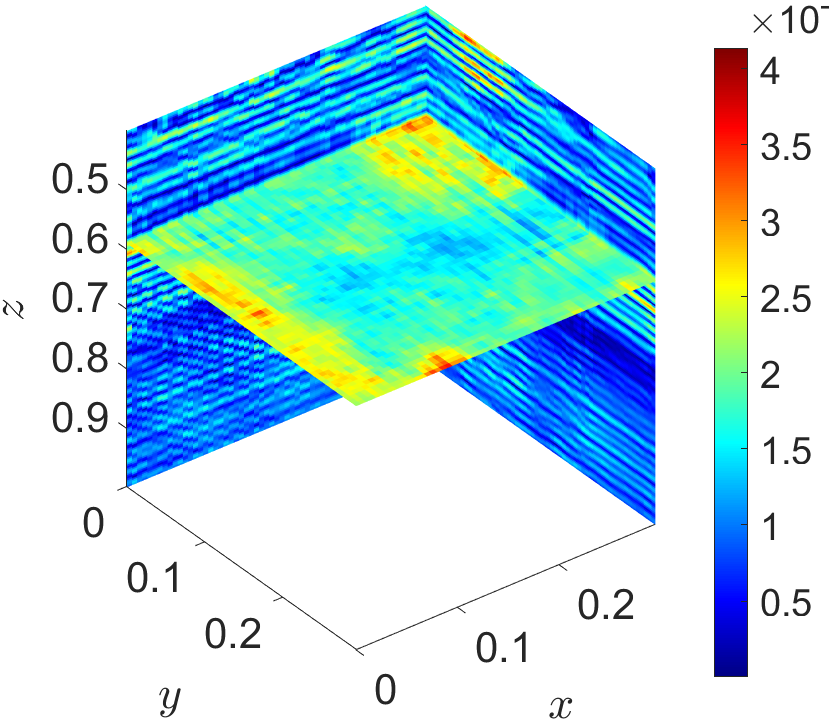
\includegraphics[width=7cm]{./image/0918.png}
     
    \caption{鉄パイプをGPRによって可視化したもの}\label{鉄パイプをGPRによって可視化したもの}
    \end{center}
    \end{figure}

 また、GPRの基本的な装置として一対の送受信アンテナを地面に照射するものがある。しかしこの場合地表全体で
多数の計測を行うため膨大な時間が必要である。ゆえに計測の時間を減らす方法が検討されてきた。そのため少ない計測点
から本来の信号を復元する圧縮センシングと呼ばれる手法が用いられる。この手法によってより少ない時間で埋設物を推定すること
ができる。加えてこの埋設物を推定する上でその物体がパイプ状でありかつ延伸の向きが分かれば、さらに探索が高速化すると考えられる。

\section{研究の目的}
 本研究の目的はガス管や水道管などの線状物体をモデル化し、偏波依存性を用いることで地中に埋設されているパイプ管の有無と向きをより少ない計測点
で推定することである。そのため偏波依存型の圧縮センシングを提案し、実験によりその有用性を検証する。

\chapter{関連技術}
\section{地中レーダの原理}



\clearpage

\begin{thebibliography}{99}
    \bibitem{radar1}M.Sato and M.Takeshita,”Estimation of subsurface fracture roughness by
    polarimetric borehole radar,” IEICE Trans. Electron., E83-C,12(2000) 1881-1888
    \bibitem{radar2}T.Moriyama, M.Nakamura, Y.Yamaguchi and H.Yamada,”Radar polarimety applied
    to the classification of target buried in the underground: Wideband Interferometric
    Sensing and Imaging Polarimetry,” Vol.3210 of Proc. of SPIE(1997) 182-189
     \bibitem{phasor}K.Oyama and A.Hirose, "Phasor Quaternion Neural Networks for Singular
     Point Compensation in Polarimetric-Interferometric
     Synthetic Aperture Radar," IEEE Transactions on Geoscience and Remote Sensing, vol. 57, no. 5, May 2019.
     \bibitem{human detection}Y.Kim, and T.Moon, "Human Detection and Activity Classification Based
     on Micro-Doppler Signatures Using Deep
     Convolutional Neural Networks," IEEE Geoscience and Remote Sensing Letters, vol. 13, no. 1, January 2016.
     \bibitem{imai}R.Imai, Y.Song, R.Natsuaki, and A.Hirose, IEEE Transactions on Geoscience and Remote Sensing,
     "Model-Based Homogeneity to Extend Compressed Sensing for Ground Penetrating Radar," vol. 60, 2022.
     \bibitem{hirose1}Y.Nakano and A.Hirose, “Improvement of plastic landmine visualization performance by use of ring-csom and frequency-domain local
     correlation,” IEICE Transactions on Electronics, vol.E92-C, no.1,
     pp.102-108, 2009.
     \bibitem{hirose2}Y.Nakano and A.Hirose, “Adaptive identification of landmine class
     by evaluating the total degree of conformity of ring-SOM,” Australian
     Journal of Intelligent Information Processing Systems, pp.22-28,2010. %http://ajiips.com.au/papers/V12.1/AJIIPS_vol12n1_26-31.pdf
    \bibitem{hirose3}R.Natsuaki and A.Hirose, “Circular property of complex-valued
    correlation learning in CMRF-based filtering for synthetic aperture
    radar interferometry,” Neurocomputing, vol.134, pp.165-172, 2014.
   %  https://www.sciencedirect.com/science/article/pii/S092523121400126X
   
    
     
     % \bibitem{jireishuu}https://geology.co.jp/archives/projects/%E5%9C%B0%E4%B8%AD%E3%83%AC%E3%83%BC%E3%83%80%E3%83%BC%E3%81%AE%E6%96%B0%E3%81%9F%E3%81%AA%E4%BA%8B%E4%BE%8B%E9%9B%86%EF%BC%88%E3%82%B1%E3%83%BC%E3%82%B9%E3%82%B9%E3%82%BF%E3%83%87%E3%82%A3%EF%BC%89#case01
   
     % \bibitem{satou}http://cobalt.cneas.tohoku.ac.jp/users/sato/newpage24.htm#:~:text=%E5%9C%B0%E4%B8%AD%E3%83%AC%E3%83%BC%E3%83%80%E3%81%AF%E9%9B%BB%E7%A3%81%E6%B3%A2,%E3%83%91%E3%83%BC%E3%82%BD%E3%83%8A%E3%83%AB%E3%83%BB%E3%82%B3%E3%83%B3%E3%83%94%E3%83%A5%E3%83%BC%E3%82%BF%E3%81%A7%E8%A8%98%E9%8C%B2%E3%81%99%E3%82%8B%E3%80%82
     % \bibitem{cs}https://www.innervision.co.jp/ressources/pdf/innervision2014/iv201409_061.pdf
    
     \end{thebibliography}

\end{document}